\subsubsection{Lung Cancer Data}
\label{sec:mv-lung}
We apply the LCC- and APC2-models that are described in Section \ref{sec:pred-mv} to the lung cancer data. The score statistics for the prediction results are displayed in Tables \ref{tbl:mv-LCC-lung} and \ref{tbl:mv-APC-lung}. We observe from the score statistics in Table \ref{tbl:mv-LCC-lung} that the LCC-models with the lowest MDSS are the models with no common effects ("No common") and with a shared period effect ("Common period"). Out of these, the "Common period"-model has a slightly lower MDSS. We observe the same trend for the different APC-models, from Table \ref{tbl:mv-APC-lung} we see that the apc- and aPc-models have the lowest MDSS. We also note that there seems to be a general trend that models with fewer shared effects out-perform models with more shared effects. We interpret this as an indication that the male and female lung cancer mortality rates have a low degree of correlation, which is a result that is in alignment with the clear difference between male and female mortality rates. 

\newpar We note that for some of the LCC-models with many common effects, \inlabru need more than 50 iterations to find a linearization. These models are the LCC-model with all effects common ("All common"), the model with common period and cohort effects ("Common period, cohort") and the model with common age and cohort effects ("Common age, cohort"). For these models, we then present the prediction results obtained after 50 iterations of the linearization, which are not necessarily the optimal predictions. Comparing these results to the converged results from the other models does then not give a completely correct picture of the difference in predictive performance. However, from Table \ref{tbl:mv-APC-lung} we observe that the corresponding APC2-models (the APC, ApC and aPC models) display a clearly higher MDSS than the APC models with fewer shared effects. Thus, we do not suspect that either of the "All common"-, "Common period, cohort"- or "Common age, cohort" LCC-models could have outperformed the LCC-models with fewer common effects.

\begin{table}
    \begin{center}
    \begin{tabular}{l |c c c }
        Model & MSE & MDSS & Contained 95\%-interval\\
        \hline
        All common          & 7.318e-8 & -17.31    & 0.9630 \\
        Common age          & 3.527e-8 & -18.48   & 0.7639 \\
        Common age, cohort  & 3.521e-8 & -16.53    & 0.7407 \\
        Common age, period  & 4.847e-8 & -18.31   & 0.8565 \\
        Common period, cohort & 1.639e-8 & -18.89    & 0.8611 \\
        Common cohort       & 1.705e-8 & -18.86  & 0.8519  \\
        Common period       & 2.198e-8 & \textbf{-19.38}   & 0.9444 \\
        No common           & 2.184e-8 & \textbf{-19.28}   & 0.9074 \\
    \end{tabular}
    \caption{Score statistics for the different multivariate LCC-models, for the lung cancer data set. The lowest mean DSS values are marked in bold font. }\label{tbl:mv-LCC-lung}
    \end{center}
\end{table}

\begin{table}
    \begin{center}
    \begin{tabular}{l |c c c }
        Model & MSE & MDSS & Contained 95\%-interval\\
        \hline
        apc    & 1.033e-8 & \textbf{-19.74}    & 0.9120 \\
        apC    & 2.437e-8 & -19.07   & 0.8843 \\
        aPc    & 1.238e-8 & \textbf{-19.83}  & 0.9028 \\
        aPC    & 7.472e-8 & -17.70   & 0.8889 \\
        Apc    & 6.709e-9 & -19.21   & 0.8981 \\
        ApC    & 1.672e-7 & -15.81   & 0.9954 \\
        APc    & 2.884e-8 & -18.71   & 0.8750  \\
        APC    & 9.055e-8 & -16.19   & 0.9676 \\
    \end{tabular}
    \caption{Score statistics for the different multivariate APC2-models, for the lung cancer data set. The lowest mean DSS values are marked in bold font. }\label{tbl:mv-APC-lung}
    \end{center}
\end{table}

\newpar A comparison of the prediction results produced with the two LCC-models and the two APC2-models with the lowest MDSS score is included in the appendix, in Figures \ref{fig:mv-LCC-lung} and \ref{fig:mv-APC-lung}.
For the two LCC-models, we observe very little difference between the two predictions. For the two APC2-models, the predictions from the apc-model seem to have slightly wider prediction intervals than the predictions from the aPc-model.

\begin{figure}
    \centering
    \begin{subfigure}[b]{.75\linewidth}
        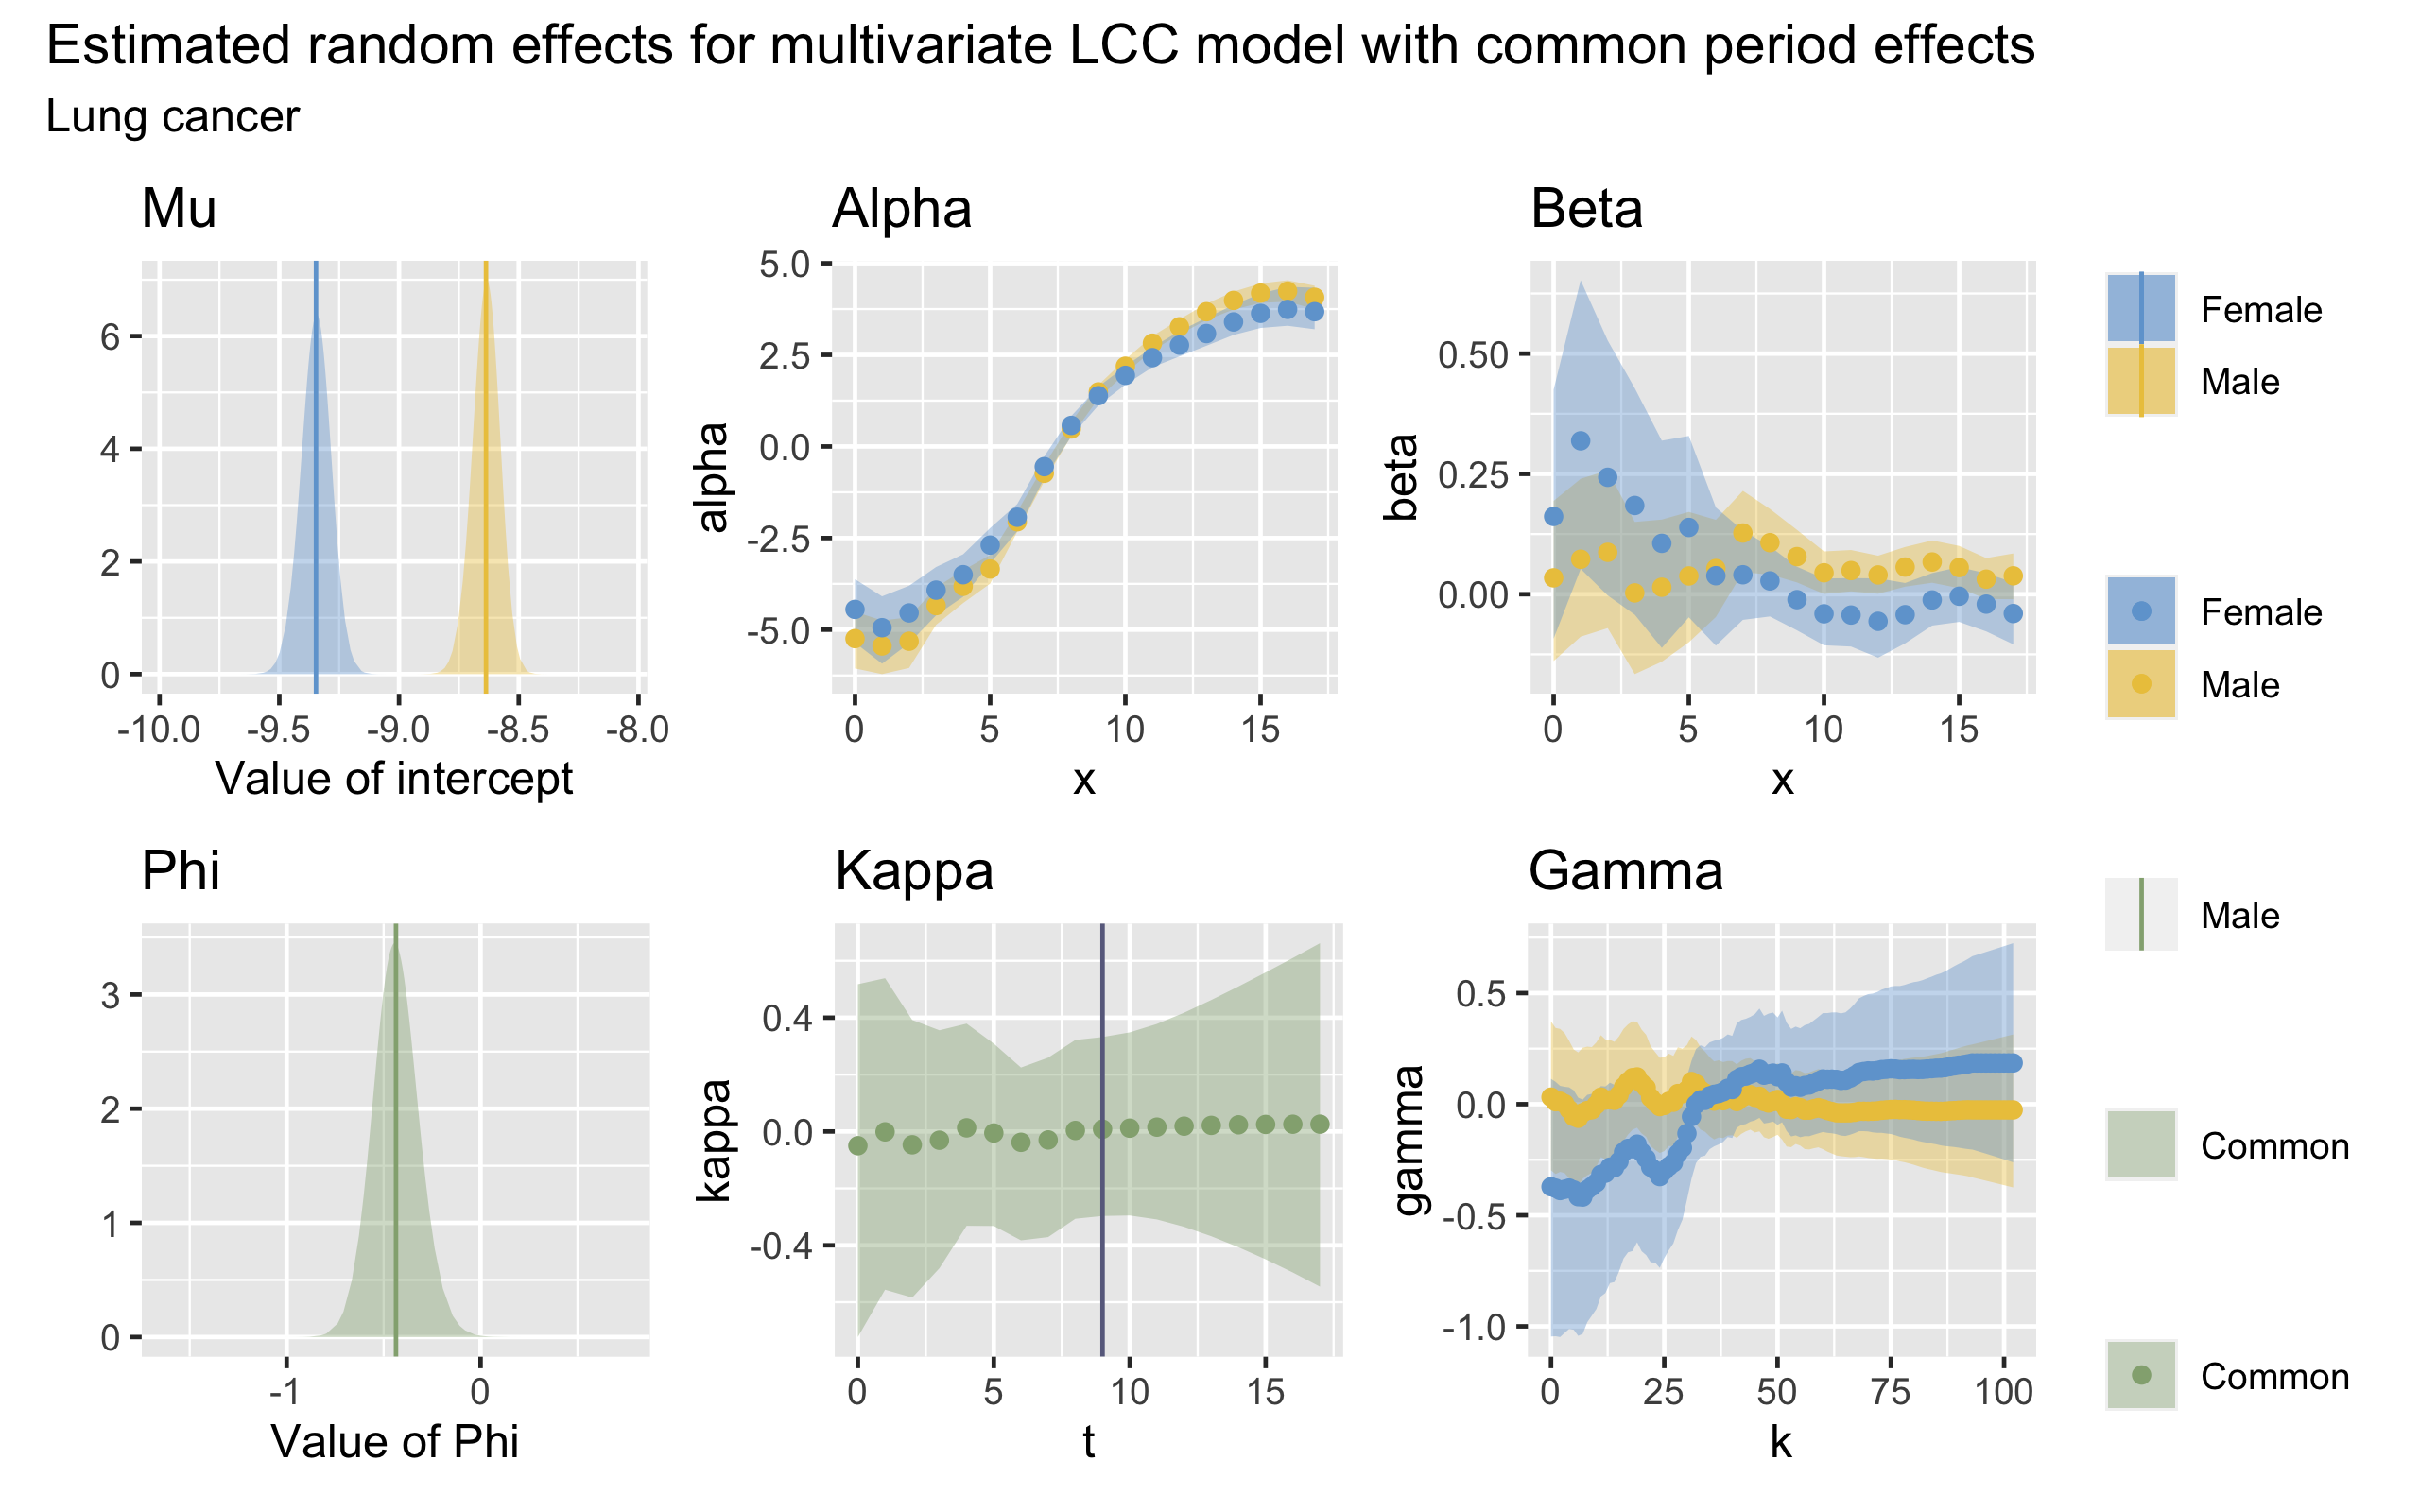
\includegraphics[width=\linewidth]{real-data/real-data-multivariate/Figures/effects-LCC-common-period-lung.png}
        \caption{The estimated overall mortality level $\mu^{\text{sex}}$ and the estimated random effects $\alpha_x^{\text{sex}}$, $\beta_x^{\text{sex}}$, $\phi$, $\kappa_t$ and $\gamma_k^{\text{sex}}$ produced with inference with the "Common period"-model.}
        \label{fig:effects-LCC-lung-top}
    \end{subfigure}
    
    \begin{subfigure}[b]{.75\linewidth}
        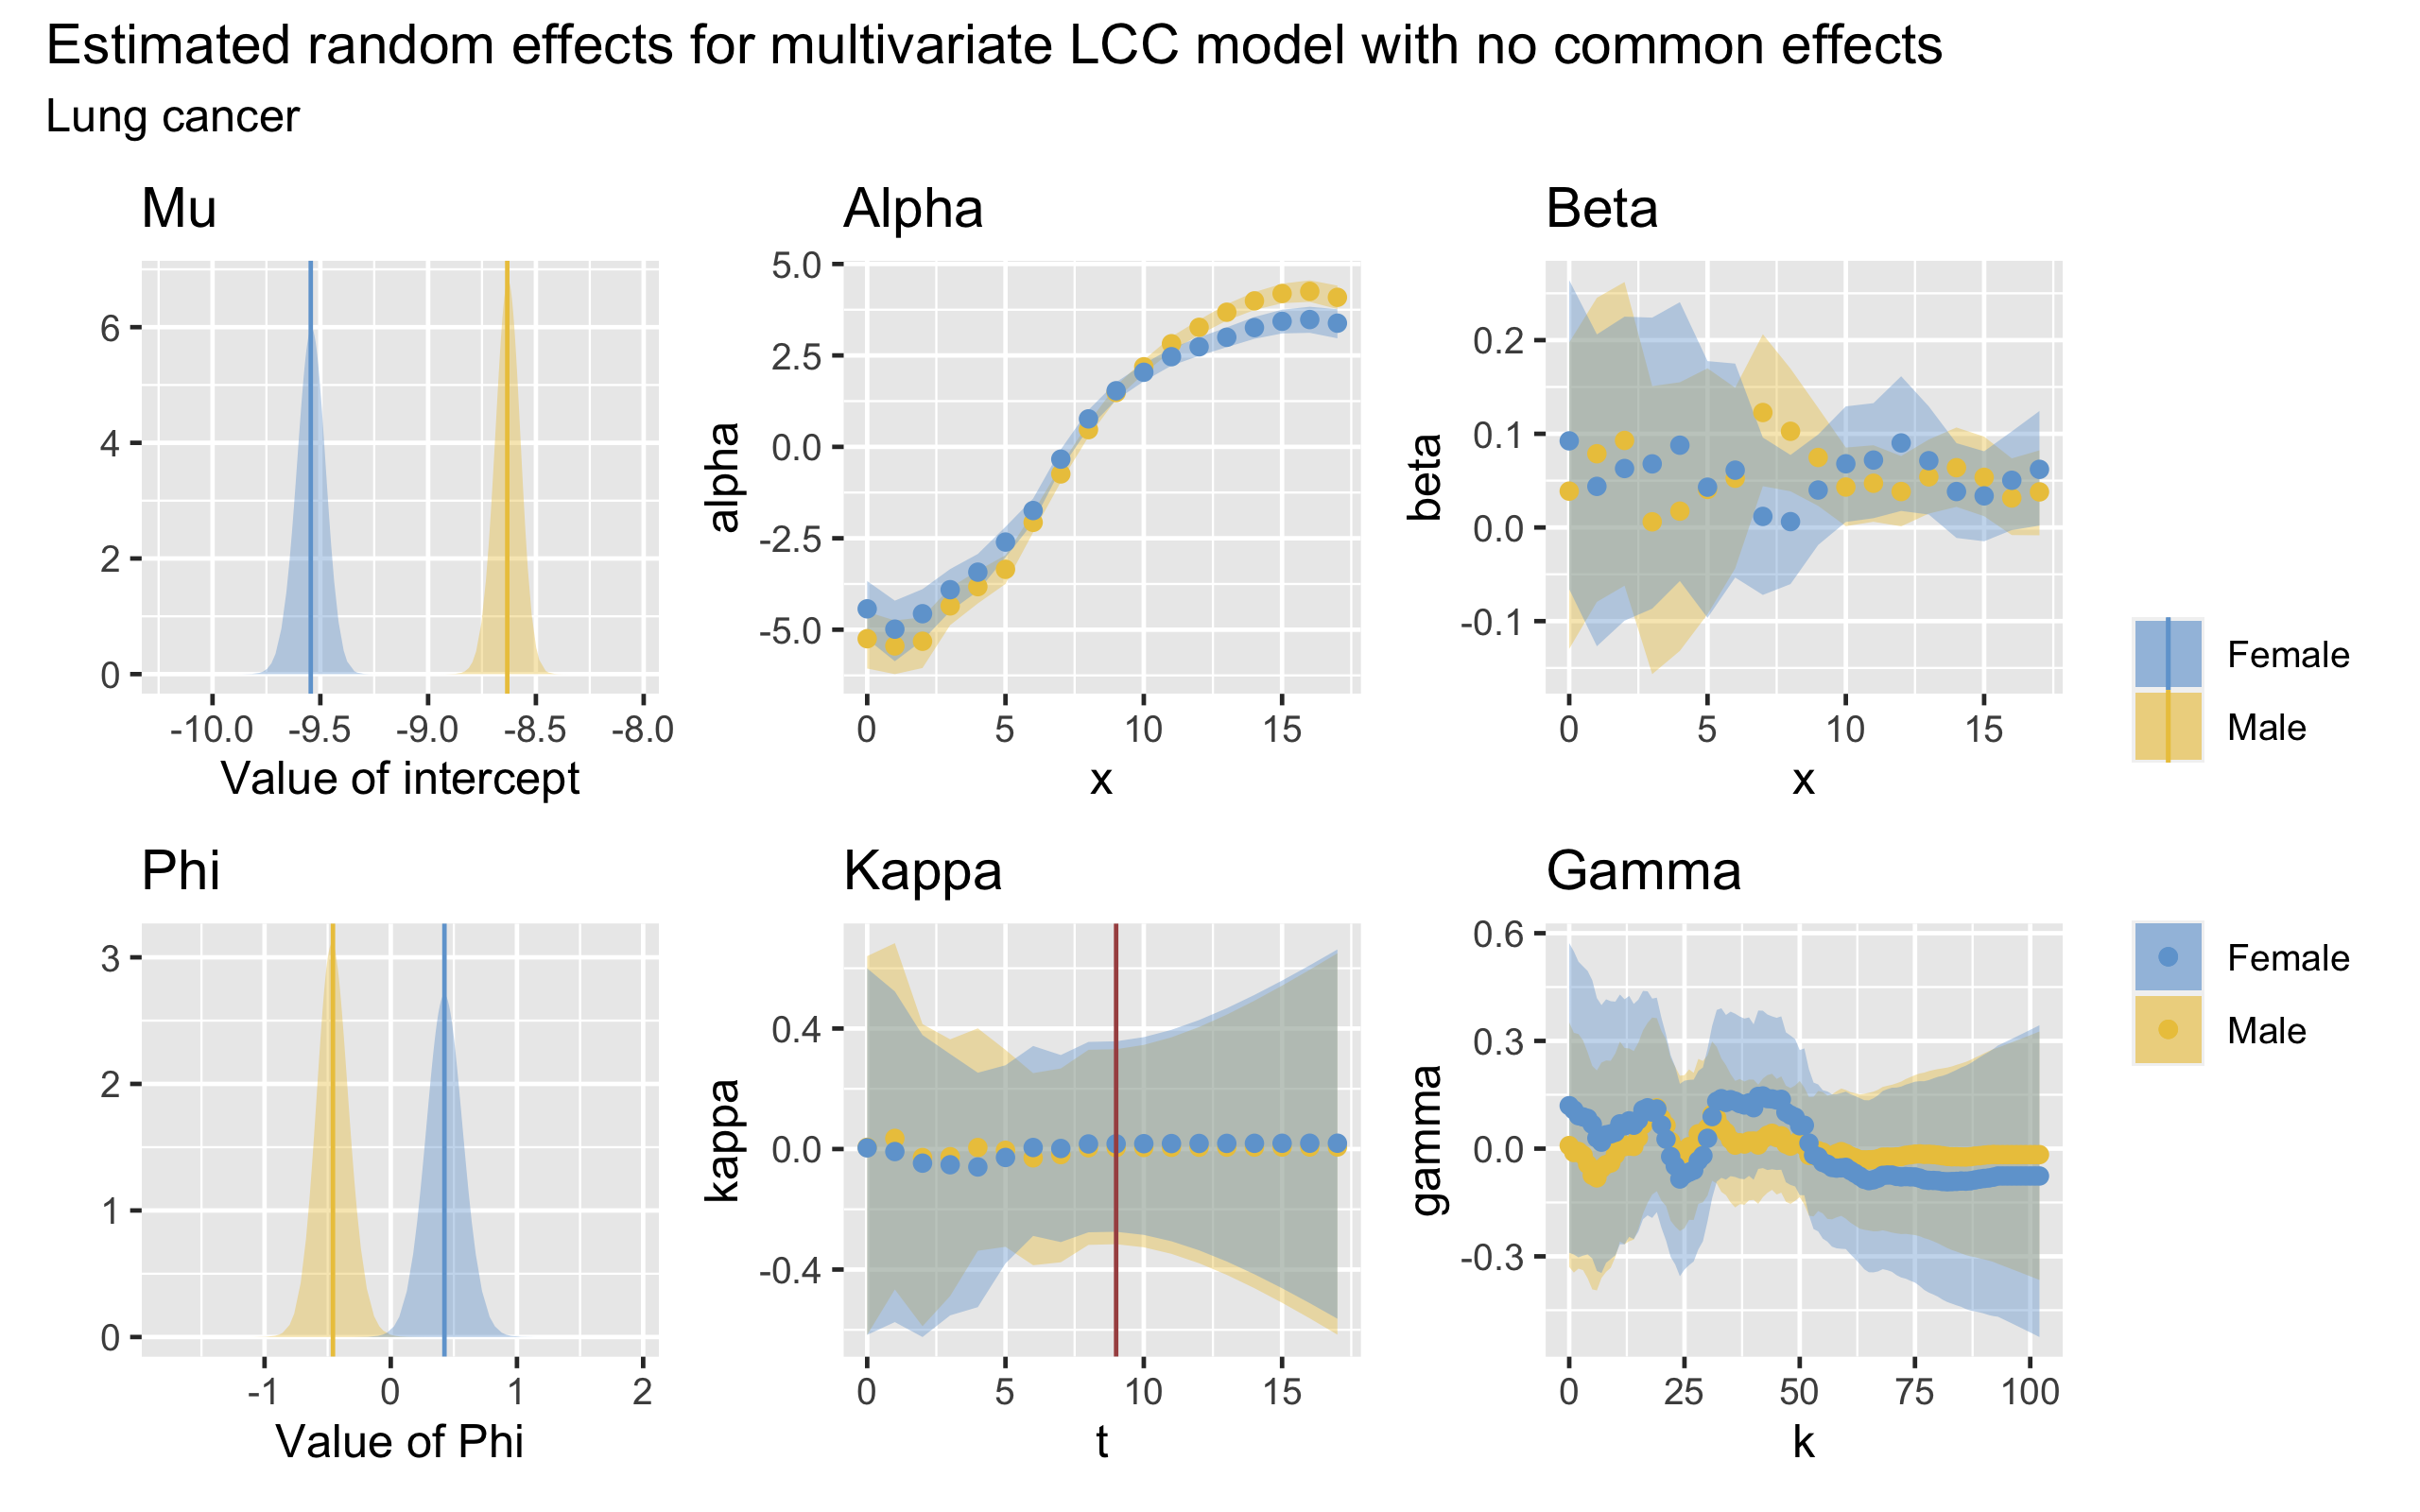
\includegraphics[width=\linewidth]{real-data/real-data-multivariate/Figures/effects-LCC-no-common-lung.png}
        \caption{The estimated overall mortality level $\mu^{\text{sex}}$ and the estimated random effects $\alpha_x^{\text{sex}}$, $\beta_x^{\text{sex}}$, $\phi^{\text{sex}}$, $\kappa_t^{\text{sex}}$ and $\gamma_k^{\text{sex}}$ produced with inference with the "No common"-model.}
        \label{fig:effects-LCC-lung-bottom}
    \end{subfigure}
    \caption{The mean values and the 95\% confidence bounds of the estimated random effects produced by inference with the "Common period" and the "No common" LCC-models on lung cancer data. The layout of the plot is similar to that of e.g. Figure \ref{fig:uv-full-data-LC-l}. The effects that are modelled as common for male and female are plotted in green, and the effects that are modelled as specific to males and females are plotted in yellow and blue, respectively. The red line marks the beginning of the predicted period. }
    \label{fig:effects-LCC-lung}
\end{figure}

\newpar Figure \ref{fig:effects-LCC-lung} displays the estimated random effects from the "No common" and the "Common period" LCC-models. For both models, the intercepts $\mu^{\text{sex}}$, the random effects $\alpha_x$ and the linear term $\phi$ seem to be clearly identified, with narrow confidence bounds. The estimated $\beta_x$ effects have clearly wider confidence bounds, especially for younger ages (low values of $x$). We note that LCC-models with very similar values for $\beta_x$, i.e. all $\beta_x = 1/X$, reduce to APC-models \parencite{Wisniowski2015}. Still, for the ages above 30 years ($x > 5$), the estimated values for $\beta_x$ are sufficiently variable and with narrower confidence bound, so we do not conclude that this is the case. For the "common period"-model, the period term $\phi$ is negative, indicating that the mortality rate decreases with time. As previously discussed, this is in line with the observed male mortality rate, but not with the female mortality rate. We observe, however, that the values of $\beta_x$ are negative for most values of $x$. This means that the sign of the slope changes for female mortality rate. We then do not interpret the good performance of the "Common period"-model as an indication of similar male and female period effects, but rather that the differences in period-specific male and female mortality rates are easily compensated by the $\beta_x$ term. For both models, the estimated mean values of $\kappa_t$ are close to zero with wide confidence bounds. This is an indication that a linear version of the LCC-models, including only the term $\phi \cdot t$ (as described in Section \ref{sec:uv-pred}) to describe the period effect might be just as good or better. 

\newpar Finally, we note that while the the estimated cohort effects $\gamma_k$ have wide confidence bounds, there are clearly observable trends in the cohort effect. For the cohorts where $k > 50$, corresponding to birth years at around year 1960 and younger, there is little variation in the cohort effect. We attribute this stabilization to the fact that these cohorts are the population that have not reached the age where they have the highest risk of getting lung cancer by 2016, so we do not have enough information to see how these cohorts will be affected differently. We also observe some of the same periodicity as discussed in Section \ref{sec:LC-full-data}. There is a clear difference in the estimated $\gamma_k$ for the models. In particular, we note that for the "Common period"-model, the estimated values for the female $\gamma_k$ are higher than the estimated male $\gamma_k$, while it is the other way around for the "No common"-model. In addition, we observe that the values of $\gamma_k$ for the "Common period"-model cover a larger range. An explanation for this might be that the "No period" model represents the period-specific differences in male and female mortality through the cohort effect $\gamma_k$ rather than through the period effect $\phi \cdot t$, such as in the "No common"-model. Finally, we observe that the $\gamma_k$ for both models displays a dip for the cohort $k \approx 25$, corresponding to birth years around 1935. This dip occurs for both male and females, but is more prominent for the male cohort effect. We recall that a similar dip is observable for the fitted effects of the univariate LCC-model, displayed in Section \ref{sec:LC-full-data}. 

\begin{figure}
    \centering
    \begin{subfigure}[b]{.75\linewidth}
        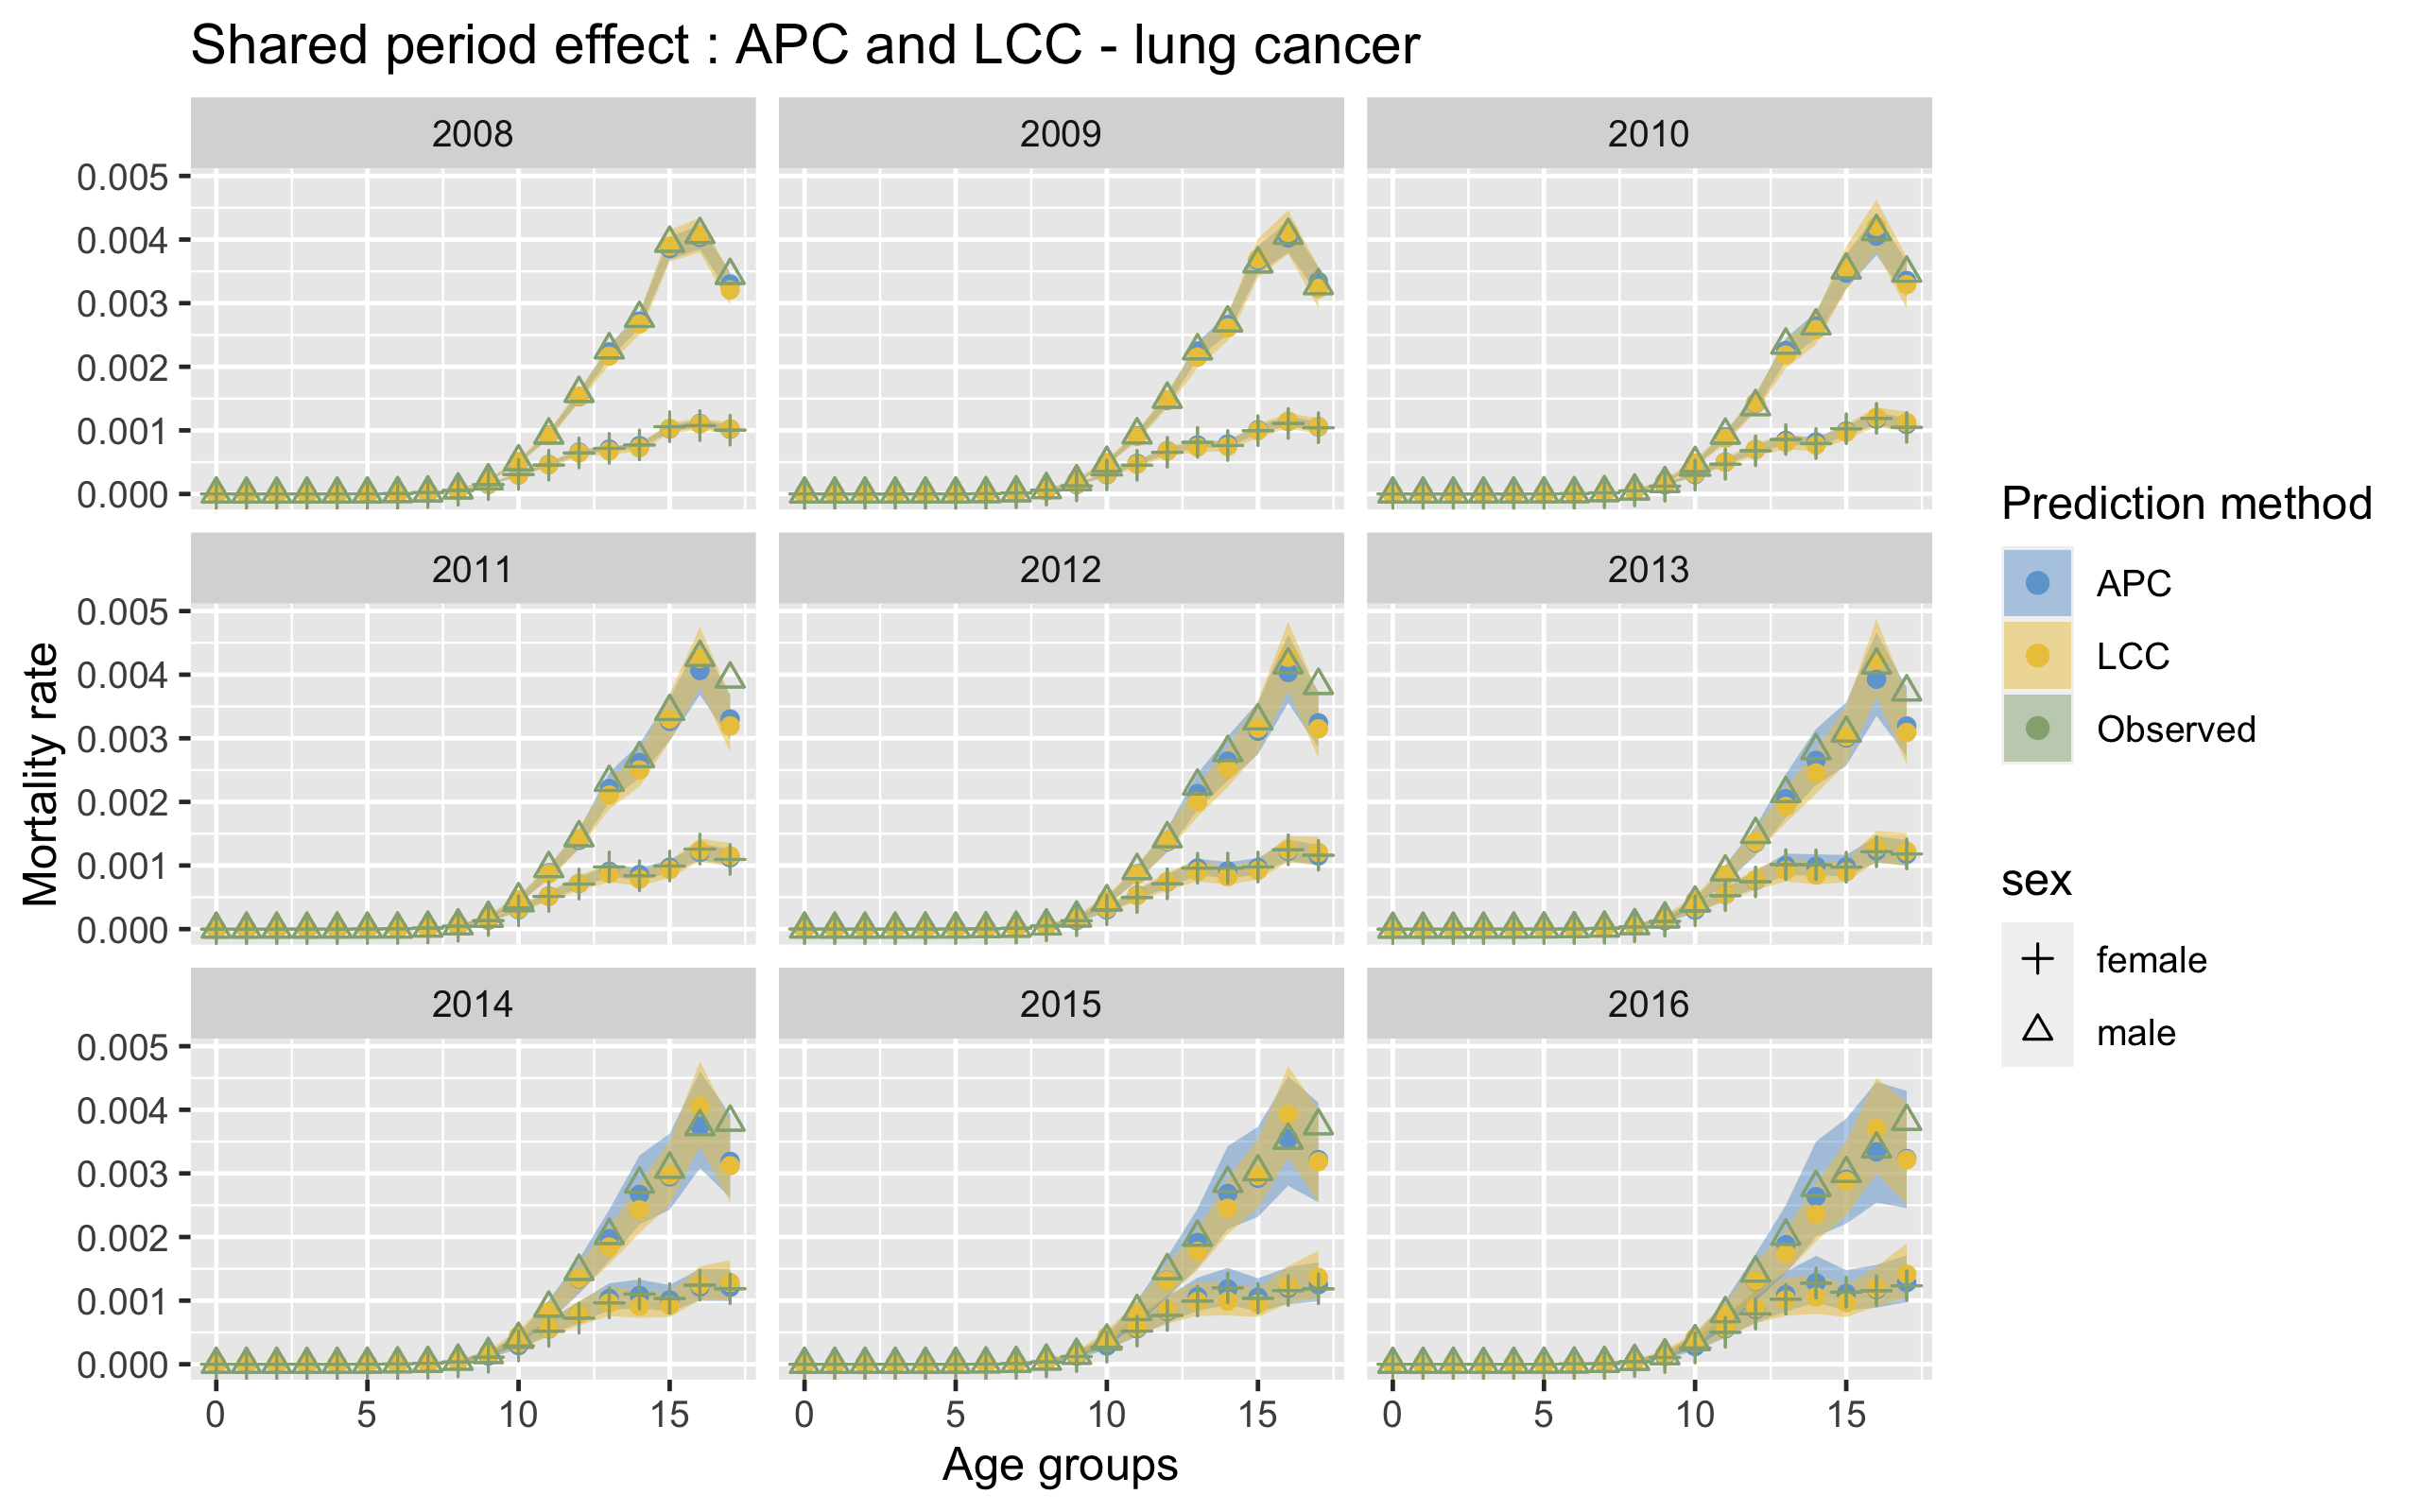
\includegraphics[width=\linewidth]{real-data/real-data-multivariate/Figures/multivariate-comparison-by-age-lung.png}
        \caption{The prediction results plotted for each of the years that were predicted, with the age groups along the horizontal axis.}
        \label{fig:mv-APC-LCC-lung-top}
    \end{subfigure}
    
    \begin{subfigure}[b]{.75\linewidth}
        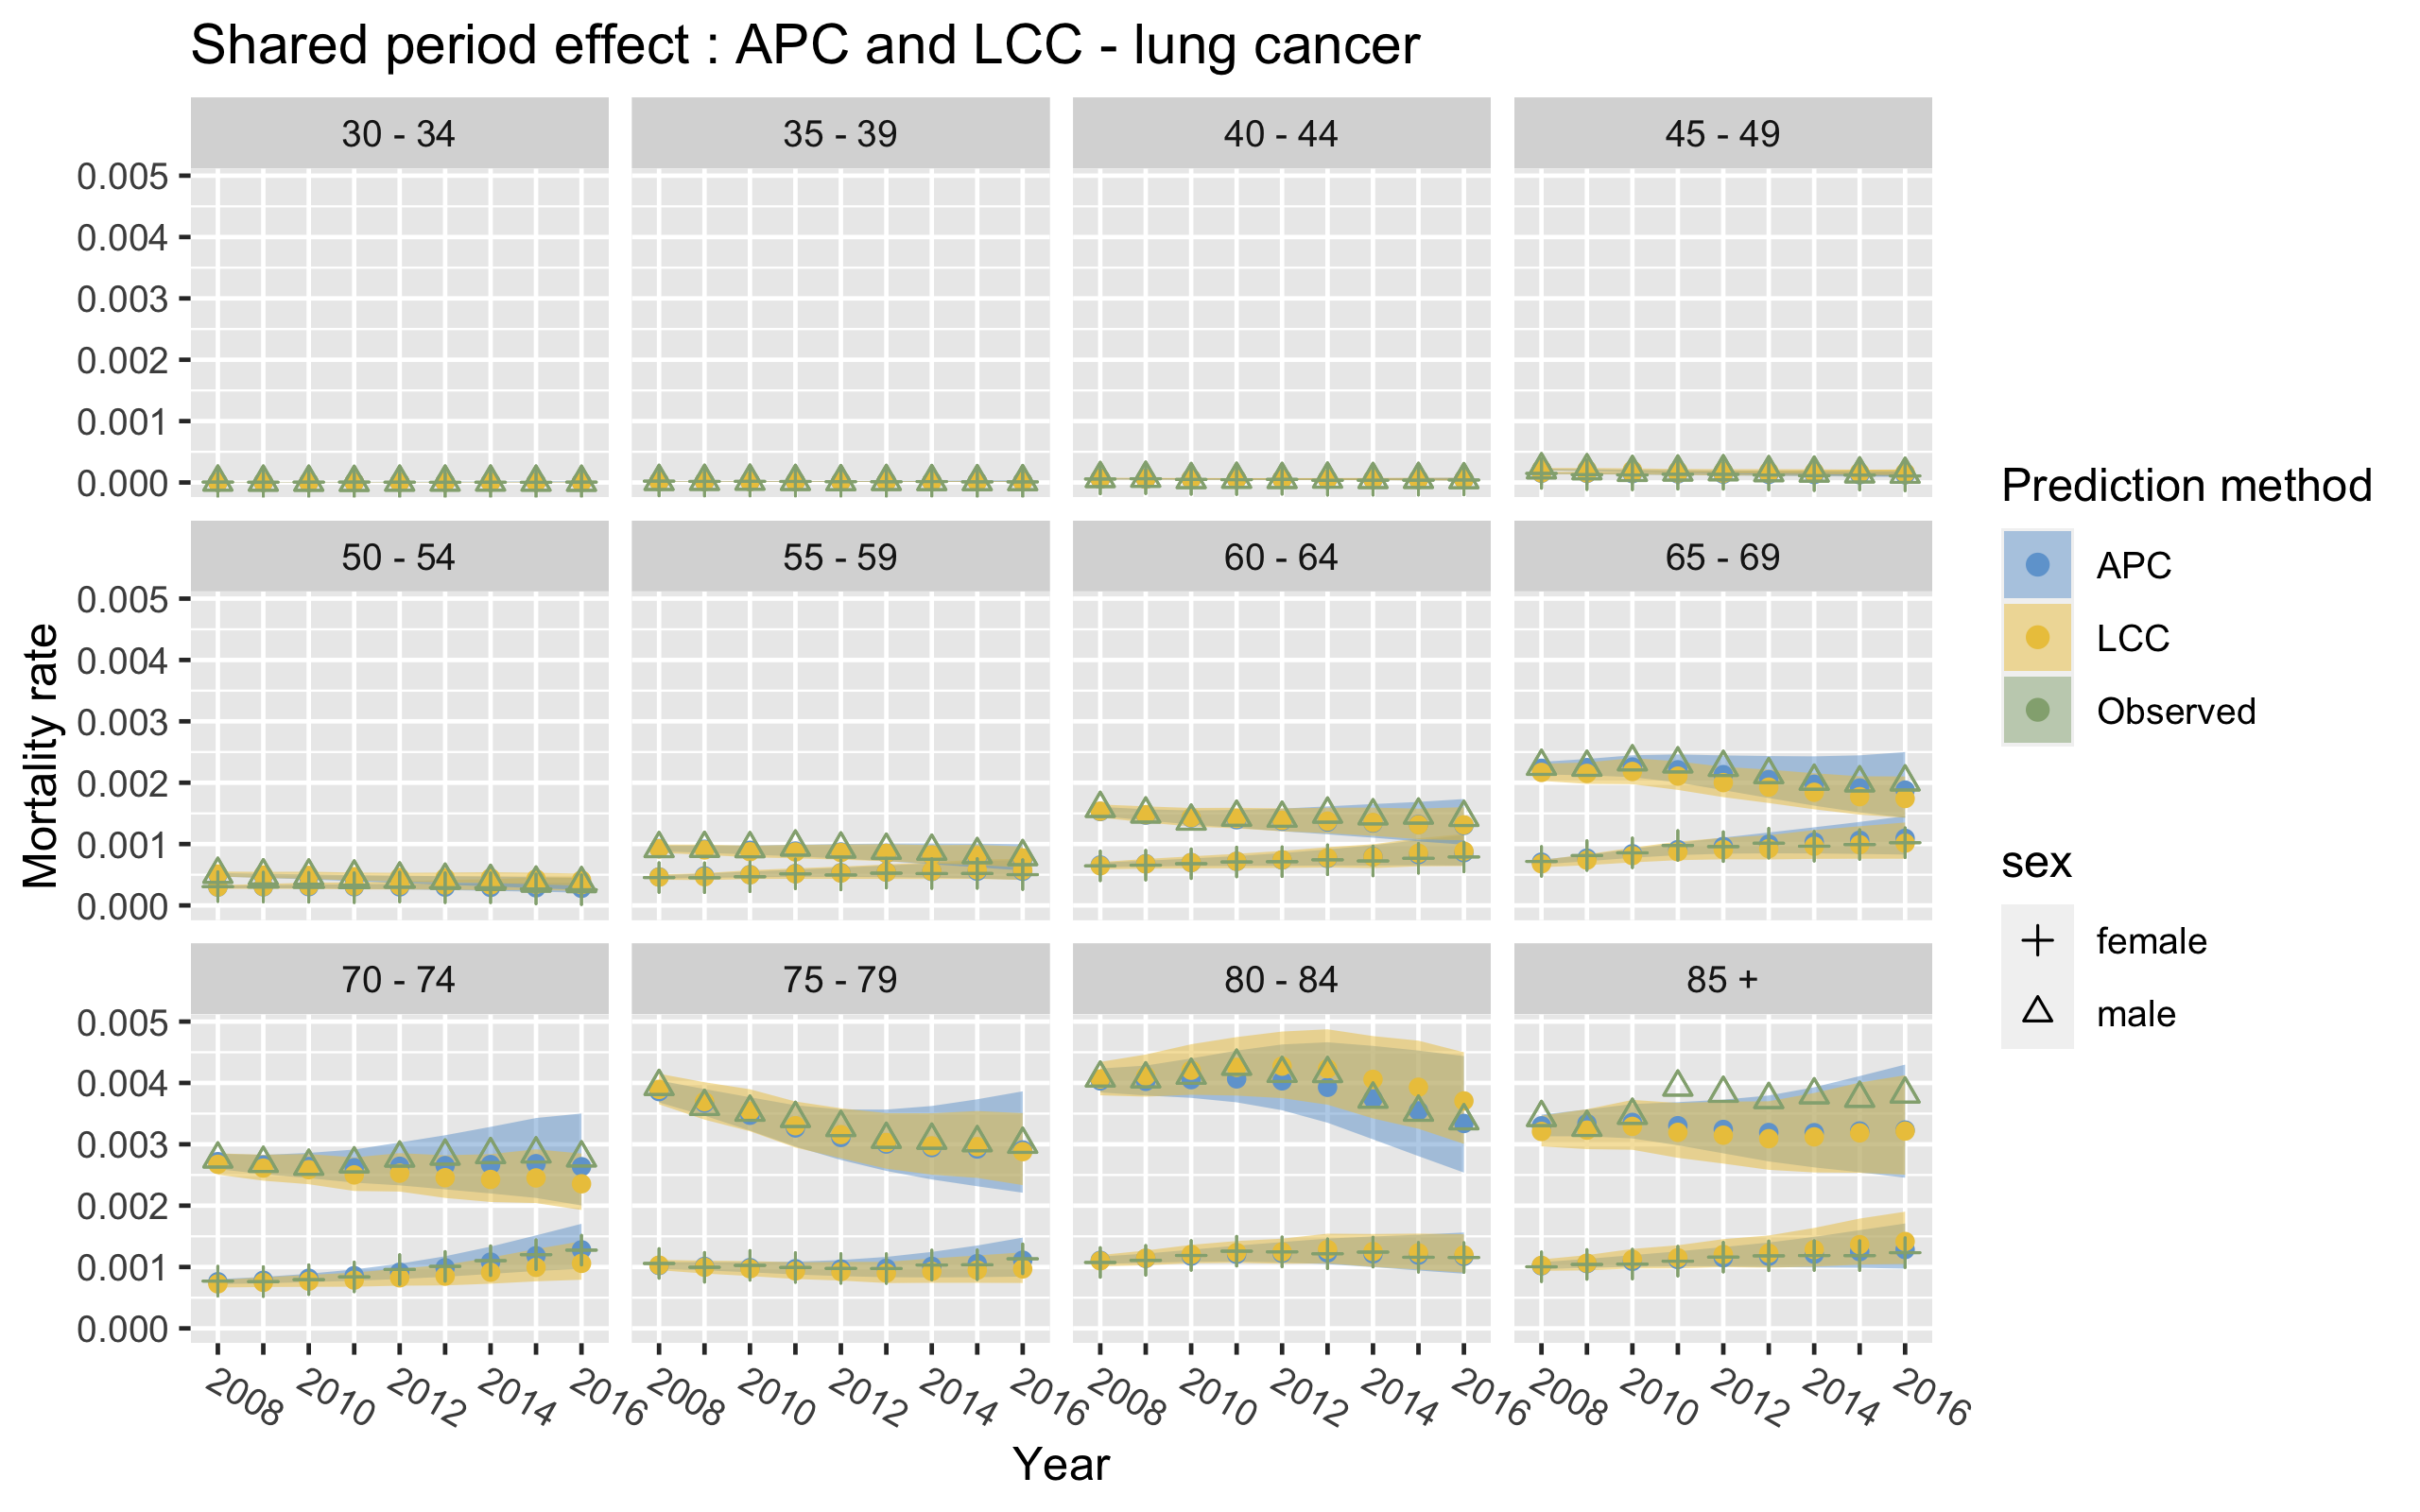
\includegraphics[width=\linewidth]{real-data/real-data-multivariate/Figures/multivariate-comparison-by-period-lung.png}
        \caption{The prediction results plotted for each age group that are 30 years and older, with the calendar years along the horizontal axis. The red line marks the beginning of the predicted periods.}
        \label{fig:mv-APC-LCC-lung-bottom}
    \end{subfigure}
    \caption{The mean values and the 95\% confidence bounds of the predicted expected lung cancer mortality rates produced by inference with the aPc-model and the "Common period"-model on data of German lung cancer (circles), together with the corresponding observed male mortality rates $Y_{x,y}^{\text{lung, male}}$ (triangles) and female mortality rates $Y_{x,y}^{\text{lung, female}}$ (crosses).}
    \label{fig:mv-APC-LCC-lung}
\end{figure}

Figure \ref{fig:mv-APC-LCC-lung} displays the prediction results from the LCC- and the APC2-models with the lowest MDSS, which are the "Common period"-model and the aPc-model, respectively. Out of these two, the aPc-model has the lowest MDSS score. From Figure \ref{fig:mv-APC-LCC-lung} we observe the same tendency as for the univariate case, that the LCC-model has slightly narrower confidence bounds. Furthermore, we see that both models predict the mortality rates for all age-groups quite well for all years, with one exception. This is the prediction of the mortality rate for males older than 85 years for the period 2010-2016, where the predictions from both models are clearly worse than for the rest.